\documentclass{extarticle}
%\usepackage{cabin}
\usepackage{mathptmx}
\usepackage{graphicx}
\usepackage[usenames, dvipsnames]{color}
\usepackage{hyperref}
\hypersetup{colorlinks = true}

	\author{
	\textbf{Viraj Karambelkar} \\
	\texttt{\href{mailto:150260003@iitb.ac.in}{\underline{150260003}}}
	\and
	\textbf{Hrishikesh T Iyer} \\
	\texttt{\href{mailto:150260023@iitb.ac.in}{\underline{150260023}}}
	\and
	\textbf{Harikrishnan KP} \\
	\texttt{\href{mailto:150260026@iitb.ac.in}{\underline{150260026}}}
	\and
	\textbf{Nitin Srirang} \\
	\texttt{\href{mailto:150260027@iitb.ac.in}{\underline{150260027}}}
	}
	\title{\color{red}\huge{Data Analysis Assignment 2}}

\begin{document}
	\maketitle
	\newpage
	\tableofcontents
	\newpage
	\section{\color{Blue} Report for Assignment 2}
	\subsection{\color{MidnightBlue} Multivariate Gaussian Distribution}
		The problem involves 2 correlated Gaussian random variables x and y with 0 mean.
		\\ Their covariance matrix is given by : \\
		$ \begin{array}{c} C \end{array} = \left [\begin{array}{c c}\sigma _{x}^{2} & \sigma _{xy} \\\sigma _{xy} & \sigma _{y}^			{2}\end{array} \right ] = \left [\begin{array}{c c} 9 & -2 \\-2 & 6\end{array} \right ] $
		\subsubsection{\color{RoyalBlue} Contour Plot}
			The contour plot obtained for the probability distribution function of x and y is : \\
			\includegraphics[scale=0.75]{contour} \\
			The contours are ellipses with their major axes inclined to the positive X axis at an obtuse angle beacause of the 				negative correlation between the two random variables. \\
			The eigenvalue equation for matrix C is $ (6-\lambda)(9-\lambda)-4=0 $ \\
			The eigenvalues are 5 and 10 for which the corresponding eigenvectors can be found. After normalization the
			eigenvectors are :

			$ \begin{array}{c} x^{'} \end{array} = \frac{1}{\sqrt{5}} \left [\begin{array}{c} 2\\-1 \end{array} \right ] $
			$ \begin{array}{c} y^{'} \end{array} = \frac{1}{\sqrt{5}} \left [\begin{array}{c} 1\\2 \end{array} \right ] $ \\
			Hence the major axes of the ellipses are along $ x+2y=0 $ and the minor axes are along $ 2x-y=0 . $

		\subsubsection{\color{RoyalBlue} 2D Histogram of random pairs generated from the distribution}
			50000 pairs of random numbers (x,y) having this distribution were generated and a 2D histogram was plotted. \\
			\includegraphics[scale=0.60]{hist} \\
			250 bins were cosidered for plotting the histogram. The height of the histogram is shown using the color scheme 			`Inferno'. \\
			The maximum number of points in the 2D histogram are towards the center (0,0) and decreases as we move outward.
			The height of the histogram at various points is clearly in agreement with the contour diagram.

		\subsubsection{\color{RoyalBlue} Distribution of z}
			A new variable z is generated for each of the 50000 pairs of x and y that are generated.
			$ z = \frac{1}{50} (6x^2 + 4xy + 9y^2) $ \\
			A histogram is plotted for the values of z. \\
			\includegraphics[scale=0.75]{hist2} \\
			The new variables x' and y' have a covariance matrix :
			$ \begin{array}{c} C' \end{array} = \left [\begin{array}{c c} 10 & 0 \\0 & 5\end{array} \right ] $
			Let a new variable w be given by
			$ w = \frac{{x'}^2}{10} + \frac{{y'}^2}{5} $
			w is a sum of squares of Gaussian distributed variables divided by the sum of their respective variances and hence 				is chi-squared distributed. On substituting values of x' and y'(i.e in terms of x and y), w simplifies to z.
			Hence z has a $ \chi^2 $ distribution which is confirmed by the histogram. \\
			The mean value of z is 2.01 with a standard deviation of 2.00.


		\newpage
	\subsection{\color{MidnightBlue} Panda Statistics}
		The weight of 100 baby pandas is read from the file \emph{"pandas.txt"} and stored in an array.
		\begin{itemize}
		\item The mean weight of the pandas is calculated to be \textbf{49.42} with an error of 				\textbf{0.32}.
		\item The size of typical fluctuations of the weight of each baby panda about the mean is an estimate of the standard 				deviation equal to \textbf{10.21}.
		\end{itemize}
		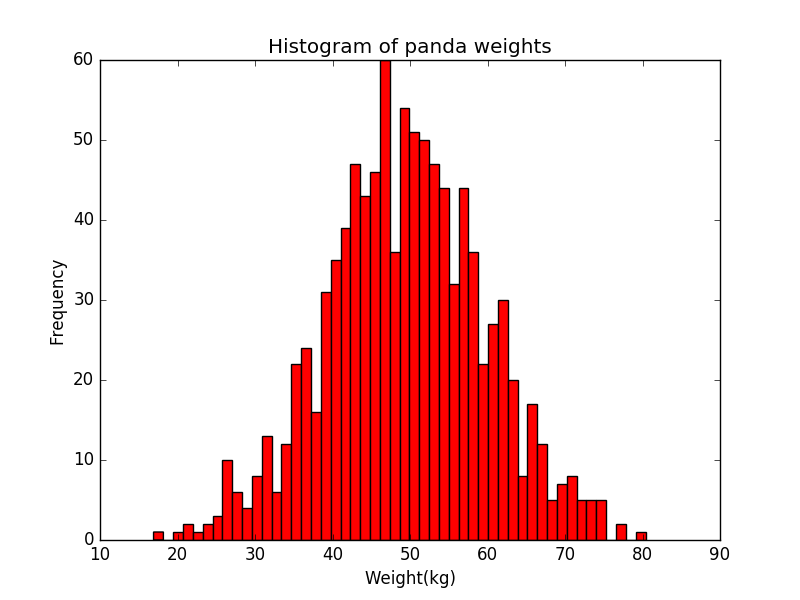
\includegraphics[scale=0.75]{panda_hist}
	
		\newpage

	\subsection{\color{MidnightBlue} Linear Expansion of Aluminium Rod}
		The readings of the length of an aluminium rod as a function of temperature is read from the file
		\emph{"linearexpansion.csv"}.
		
		\subsubsection{\color{RoyalBlue} Scatter Plot}
		The scatter plot obtained for the given data is: \\
		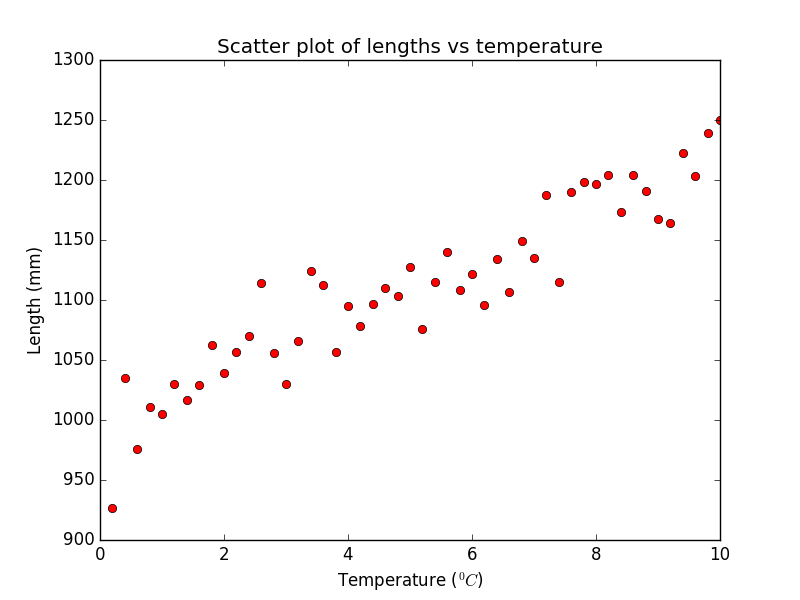
\includegraphics[scale=0.75]{scatter} \\
		
		\subsubsection{\color{RoyalBlue} Best Fit Line}
		Let us consider y=mx+c as the equation for the best-fit line. Analytically the value of m and c can be found: \\
		$ SS = \sum_{i=0}^{n}(y_{i}-(mx_{i}+c))^{2} 
		$
		\\ \\
		where SS is the sum of squares. \\ \\
		$
		\frac{\partial SS}{\partial m} = 0
		\Rightarrow  \sum_{i=0}^{n} x_{i}(y_{i}-(mx_{i}+c)) = 0 \\ \\
		\frac{\partial SS}{\partial c} = 0 
		\Rightarrow  \sum_{i=0}^{n} (y_{i}-(mx_{i}+c)) = 0 \\ \\
		\sum_{i=0}^{n} y_{i} = m\sum_{i=0}^{n} x_{i} + Nc \\ \\
		\Rightarrow c = \overline{y} - m\overline{x} \\ \\
		\sum_{i=0}^{n} x_{i}y_{i} = m\sum_{i=0}^{n} x_{i}^{2} + Nc\overline{x} \\ \\
		\sum_{i=0}^{n} x_{i}y_{i} = m\sum_{i=0}^{n} x_{i}^{2} + N\overline{x}(\overline{y}-m\overline{x}) \\ \\
		m = \frac{\sum_{i=0}^{n} x_{i}y_{i} - \overline{x} \sum_{i=0}^{n} y_{i}} {\sum_{i=0}^{n} x^{2}_{i} - N\overline{x}^{2}} \\ 
		$
		\\
		The error expected on the extrapolated length is: \\
		$
		\quad \sigma  = \sqrt{\frac{1}{N-2} \sum_{i=0}^{n} (y_{i}-\hat y)^{2}} \\ \\
		$
		where $ \hat y = mx_{i}+c. $ \\ \\
		Let $ \sigma $ be the single measurement error for each y \\
		$
		 \sigma ^{2}_{m} = \frac{\sum_{i=0}^{n} ((x_{i} - \overline{x})^{2} \sigma^ {2}_{yi}} {\sum_{i=0}^{n} {x_{i}^{2} -
		 N\overline{x}^{2}}^{2}} \\ \\
		\sigma ^{2}_{m} = \frac{\sigma ^{2}} {(\sum_{i=0}^{n} x^{2}_{i}) - N\overline{x}^{2}} \\ \\
		c=\frac{\sum_{i=0}^{n} y_{i}}{N} - m\overline{x} \\ \\
		\sigma ^{2}_{c} = \frac{1}{N^{2}} \sum_{i=0}^{n}(\sigma _{yi}^{2} + \overline{x} ^{2} \sigma ^{2}_{m}) \\ \\
		\sigma ^{2}_{c} = \frac{\sigma ^{2}}{N} + \overline{x} ^{2} \sigma ^{2}_{m} \\ \\
		$
		
		
		
		\begin{itemize}
		\item The value of m obtained is \emph{22.90} which is $ \alpha $, the coefficient of linear expansion in units mm/K. This 				value is reported with an error of \emph{3.56 mm/K}.
		\item The value of c obtained is \emph{993.51} which is the estimate of the length of rod at $ 0^{\circ}C $ in mm.
		\item Linear extrapolation upto $ 15^{\circ}C $ gives an expected length of \emph{1337.04 mm}.
		\item Error in length at $ 15^{\circ}C $ is \emph{26.71 mm}.
		\end{itemize}
		
		\newpage
		The best fit line obtained has been plotted over the scatter diagram. \\ 		
		\includegraphics[scale=0.75]{bestfit} \\


		\newpage

	\section{\color{Blue} Summary}
		\subsection{\color{MidnightBlue} Problem 1}
		\begin{itemize}
		\item Based on given data a contour plot was made for the probability distribution function of x and y.
		\item Random pairs of numbers x and y having this distribution were generated and a 2D histogram plotted.
		\item A variable $ z = \frac{{x'}^2}{10} + \frac{{y'}^2}{5} $ is generated for each of these pairs and a histogram plotted.
		\item z has a $ \chi ^{2} $ distribution with mean value \emph{2.01} and error \emph{2.00}.
		\end{itemize}
		
		\subsection{\color{MidnightBlue} Problem 2}
		\begin{itemize}
		\item A histogram has been plotted for the weight distribution among the different baby pandas.
		\item Mean weight of pandas is \emph{49.42 kg} with an error of \emph{0.32 kg}. The typical 					fluctuation about this mean is \emph{10.21}.
		\end{itemize}
		
		\subsection{\color{MidnightBlue} Problem 3}
		\begin{itemize}
		\item A scatter plot has been made for the variation of length with temperature.
		\item The best fit line is found by analytical methods. The coefficient of linear expansion is estimated to be 
			\emph{22.90} mm/K with error \emph{3.56 mm/K} and the length of rod at $ 0^{\circ}C $ to be \emph{993.51 mm}.
		\item By extrapolation, the length of rod at $ 15^{\circ}C $ is estimated to be \emph{1337.04 mm}.
		\item Error in Length at $ 15^{\circ}C $ is \emph{26.71 mm}.
		\end{itemize}
		
		\newpage
		
	\section{\color{Blue} Team Responsibilities}
		The roles for the group members for this assignment are as follows:
		\begin{center}
		\begin{tabular}{|c|c|}
		\hline
		Nitin Srirang & Group Leader \\
		\hline
		Hrishikesh T Iyer & Coder \\
		\hline
		Viraj Karambelkar & Web Manager \\
		\hline
		Harikrishnan KP & Report Writer \\
		\hline
		\end{tabular}
		\end{center}

	\section{\color{Blue} Website}
		The link to our website is \href{https://thewimpykids.wordpress.com}{The WIMPy Kids-Bringing Numbers to Life}. The 			code and report for each week's assignment can be found on this site. The code has also been uploaded on Github, the link 			for the assignment repository is \href{https://github.com/The-WIMPy-Kids/Data-Analysis-Assignment.git}{Data Analysis 			Assignment Repo}. The code for this week's assignment is in this
		\href{https://github.com/The-WIMPy-Kids/Data-Analysis-Assignment/tree/analytical}{branch} of the repository.




\end{document}
